\documentclass[a4paper]{article}
\usepackage[utf8]{inputenc}
\usepackage{amsmath}
\usepackage{amssymb}
\usepackage{mathtools}
\usepackage{amsfonts}
\usepackage{lastpage}
\usepackage{pdfpages}
\usepackage{fancyvrb}
\usepackage[table]{colortbl}
\usepackage{fancyhdr}
\usepackage[linesnumbered, ruled]{algorithm2e}
\usepackage{graphicx}
\SetKwRepeat{Do}{do}{while}%
\usepackage[margin=2.5 cm]{geometry}


\pagestyle{fancy}
\cfoot{Page \thepage\ of \pageref{LastPage}}
\DeclareGraphicsExtensions{.pdf,.png,.jpg}
\author{Siggi Arnason (5961181) \\ Victor Petren Bach Hansen (5990025)}
\title{Algorithms \& Networks \\ Exercise 2}
\lhead{Algorithms \& Networks}
\rhead{Exercise 2}

\begin{document}
\maketitle
\section{Stable Roommates}
In our instance of the stable roommates problem, we seek an assignment such that the preference list below is abided:
\begin{center}
    \begin{tabular}{ | c || c  c  c  c  c  c  c |}
          \hline
              1: & 2 & 5 & 4 & 6 & 7 & 8 & 3 \\
              2: & 3 & 6 & 1 & 7 & 8 & 5 & 4 \\
              3: & 4 & 7 & 2 & 8 & 5 & 6 & 1 \\
              4: & 1 & 8 & 3 & 5 & 6 & 7 & 2 \\
              5: & 6 & 1 & 6 & 2 & 3 & 4 & 7 \\
              6: & 7 & 2 & 5 & 3 & 4 & 1 & 8 \\
              7: & 8 & 3 & 6 & 5 & 1 & 2 & 5 \\
              8: & 5 & 4 & 7 & 1 & 2 & 3 & 6 \\
          \hline
    \end{tabular}
\end{center}
We find such an assignment using the algorithm described in the lecture. The algorithm is divided into 3 phases, where we start of by proposing and filtering out candidates.\\

We get the following sequence of proposals, which takes place according to the rules of the algorithm:
\begin{align*}
  \mbox{$1$ proposes to $2$;}& &\mbox{$2$ holds $1$}\\
  \mbox{$2$ proposes to $3$;}& &\mbox{$3$ holds $2$}\\
  \mbox{$3$ proposes to $4$;}& &\mbox{$4$ holds $3$}\\
  \mbox{$4$ proposes to $1$;}& &\mbox{$1$ holds $4$}\\
  \mbox{$5$ proposes to $6$;}& &\mbox{$6$ holds $5$}\\
  \mbox{$6$ proposes to $7$;}& &\mbox{$7$ holds $6$}\\
  \mbox{$7$ proposes to $8$;}& &\mbox{$8$ holds $7$}\\
  \mbox{$8$ proposes to $5$;}& &\mbox{$5$ holds $8$}\\
\end{align*}
The proposal algorithm terminates and we finish phase 1 with filtering out candidates from the preference list. As we can see from the proposals above, we get no rejections and we are unable to eliminate due to someone holding a better proposal. We can therefore only remove those that are worse than the current proposal. We get the filtered list (current proposals are marked in bold):
\begin{center}
    \begin{tabular}{ | c || c  c  c |}
          \hline
          1: & 2 & 5 & \textbf{4} \\
          2: & 3 & 6 & \textbf{1} \\
          3: & 4 & 7 & \textbf{2} \\
          4: & 1 & 8 & \textbf{3} \\
          5: & 6 & 1 & \textbf{6} \\
          6: & 7 & 2 & \textbf{5} \\
          7: & 8 & 3 & \textbf{6} \\
          8: & 5 & 4 & \textbf{7} \\
          \hline
    \end{tabular}
\end{center}
We now enter phase 2, where we can identify the following all-or-nothing cycles:
  $$ 1,8,3,6 $$
  $$ 2,5,4,7 $$
We can now once again filter the preference list by letting each $b_i$ reject the current proposal from $a_i$, let $a_i$ propose to $b_{i+1}$ and remove preferences that occur after $b_{i+1}$. Applying this for both cycles, results in the following reduced preference list:
\begin{center}
    \begin{tabular}{ | c || c  c  |}
          \hline
          1: & 2 & \textbf{5} \\
          2: & 3 & \textbf{6} \\
          3: & 4 & \textbf{7} \\
          4: & 1 & \textbf{8} \\
          5: & 6 & \textbf{1} \\
          6: & 7 & \textbf{2} \\
          7: & 8 & \textbf{3} \\
          8: & 5 & \textbf{4} \\
          \hline
    \end{tabular}
\end{center}
Where we can see that we get the following matching:
  $$ S=(1,5)(2,6)(3,7)(4,8) $$
which is a stable roommates assignment.

\section{Arbitrage}
\subsection*{a)}
We can model the problem as a complete graph $G=(V,E)$ on $n=|V|$ vertices, where vertex $c_i$ corresponds to currency $i$ and an edge $(i,j)\in E$ corresponds to exchanging from currency $i$ to $j$.

We know that in order to make a profit on a sequnce of currency exchanges, $c_1, c_2, \ldots, c_r$, we must have that:
$$
  R(1,2)*R(2,3)*\ldots*R(r,1)> 1
$$
We can take the logarithm of both sides of the equation, which gives us that
$$
  \log R(1,2) + \log R(2,3)+\ldots+\log R(r,1)> 0
$$
If we assign the cost of going from currency $c_i$ to $c_j$ to $\log R(i,j)$, the arbitrage problem can be seen as to indentify a positive cycle in the graph. We could also assign the cost to $-\log R(i,j)$, which changes to problem into finding a negative cycle in the graph, which is a very known problem.
\subsection*{b)}
We know that the Bellman-Ford algorithm can be used to identify negative cycles, so if we model the problem as states in the previous task, we can run the Bellman-Ford algorithm, and if it returns that there exists a negative cycle, we are done.

Bellman-Ford runs in $\mathcal{O}(|V|*|E|)$ time and seeing as the graph is complete, we have $(n-1)^2=\mathcal{O}(n^2)$ edges, which gives a total running time of $\mathcal{O}(n^3)$.
\section{Flows with lower bounds}
The method of solving the maximum flow problem with lower bounds on capacities, stated in the lecture, is as follows:
\begin{enumerate}
    \item Add edge $(t,s)$ to obtain $G'$
    \item Add new supersource and supersink, $s'$ and $t'$
    \item Change edges according to slides in order to obtain $G''$
    \item Compute max-flow in $G''$
    \item Ignore $s'$ and $t'$ to translate back to adm. circulation in $G'$
    \item Ignore the edge $(t,s)$ to translate back to adm. flow in $G$
    \item Compute $G_f$
    \item Compute max-flow $f'$ in $G_f$ with flow algorithm
    \item Output $f+f'$
\end{enumerate}
Step 1 and 2 both takes $\mathcal{O}(1)$ time, step 3 takes $\mathcal{O}(m)$ time, step 4 takes $\mathcal{O}(n^3)$ time, step 5 and 6 both take $\mathcal{O}(1)$ time, step 7 and 8 takes $\mathcal{O}(n^3)$ time and step 9 takes $\mathcal{O}(1)$. This gives us a total running time of $\mathcal{O}(n^3+m)$ time.
\section{Escape problem}
\subsection{}
We can restructure the graph $G=(V,E)$, so it becomes a question of solving the ordinary max-flow problem. In order to do this, we can eliminate the vertex capacities by, for each vertex, introduce another vertex and edge, such that for a vertex $v_i$ with incomming edges $(l_1,i), \ldots, (l_x)$  and outgoing edges $(i,k_1),\ldots, k_y$, we get vertices $v_{i1}$ and $v_{i2}$ and edges $(l,i1)$, $(i1,i2)$, $(i2,l)$.

We can call this newly obtained graph $G'=(V', E')$, which has the size $|V'|=2|V|= \mathcal{O}(n)$ and $|E'|=|V|+|E|=\mathcal{O}(n+m)$.
\subsection{}
We propose the following algorithm to solve the escape problem:
\begin{enumerate}
  \item Add supersource $s$ and connect it to the $m$ starting points
  \item Add supersink $t$ and connect it to the $4(n-2)+4=4n-4$ possible end points
  \item Let undirected edges become directed, one in each directed. e.g. for each undirected edge $(i,j)\in E$, we get the directed edges $(i,j)$ and $(j,i)$.
  \item Assign a capacity of $1$ to all edges and vertices
  \item Use the graph restructuring method described previously to obtain an ordinary max flow problem
  \item Solve the max flow problem with your favorite max-flow algorithm
  \item If the resulting flow $f$ is equal to $m$, then the flow will correspond to a solution to the escape problem
\end{enumerate}
The problem can be solved using the Edmonds-Karp algorithm, which runs in $\mathcal{O}(VE^2)$ time. In our problem, we have that the number of edges is: $m$ from the source to the starting points, $4n-4$ from the endpoints to the sink, $2(2n^2-2n)$ edges inside the grid in the directed case, which gives a total of $\mathcal{O}(n^2)$ edges. The total number of vertices are $n^2+2=\mathcal{O}(n^2)$. With the Edmonds-Karp algorithm, the total runtime then becomes
$\mathcal{O}(VE^2)=\mathcal{O}(n^2n^{2^2})=\mathcal{O}(n^6)$
\section{Modelling phasing out capital equipment}
Infinite capacity for all edges. Lower bounds $l(d_1)$, ..., $l(d_p)$ shown on graph. $s_{p+1}$ is the price in the end of year p. Run minimum cost flow algorithm for the number of ships the company has in the beginning.\\
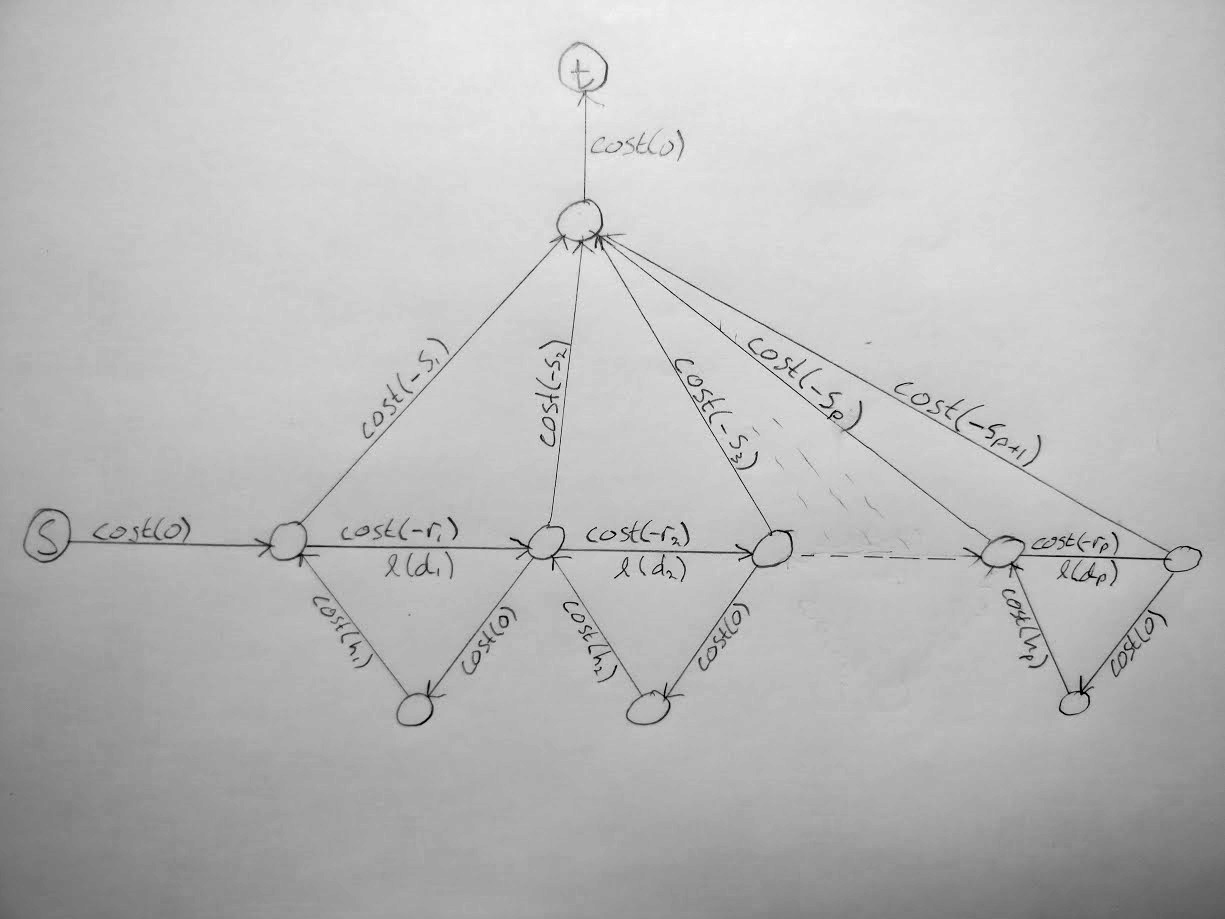
\includegraphics[width=\textwidth]{nr5graph}

\section{Bonus question: Spacecraft computer games}
We look at the corridor as a grid system and treat it as a graph G(V,E). We modify Dijkstra's algorithm so that the distance from the source to a vertex v is the number of towers that needs to be destroyed to travel that path. We keep track of what towers the shortest known path to a vertex needed to be destroyed with $destroyedTowers$. \\
After the algorithm is run, dist[end vertex] gives the minimum number of towers that need to be destroyed to get there and destroyedTowers[end vertex] gives the vertices that need to be destroyed.
\begin{algorithm}[H]
  \KwData{Graph $G(V,E)$, starting vertex $source$}
  \KwResult{The minimum number of towers the need to be destroyed to get from $source$ to each vertex, and the towers that need to be destroyed. }
  
  create vertex set $Q$\;
  \ForEach{vertex $v$ in $Graph$}{
  	$dist[v]$ = INFINITY\;
  	$destroyedTowers[v]$ = EMPTY SET\;
  	$guardingTowers[v]$ = EMPTY SET\;
  	add $v$ to $Q$\;
  }
  
  \ForEach{vertex $v$ in $Graph$}{
  	\If{$v$ has a tower}{
  		$guardingTowers[v].add(v)$\;
  		\ForEach{vertex $u$ within tower range from $v$}{
			$guardingTowers[u].add(v)$\;	
  		}
  	}
  }
  
  $dist[source]$ = 0\;
  \While{$Q$ is not empty}{
  	$u$ = vertex in $Q$ with min $dist[u]$\;
  	remove $u$ from $Q$\;
  	
  	\ForEach{neighbor $v$ of $u$}{
  		$altDestroyedTowers$ = $unionSet(destroyedTowers[u],guardingTowers[v])$\;
  		$alt$ = size of $altDestroyedTowers$\;
  		\If{$alt < dist[v]$}{
  			$dist[v]$ = $alt$\;
  			$destroyedTowers[v]$ = $altDestroyedTowers$\;
  		}
  	}
  }
  	\Return{dist, destroyedTowers}
    
  \caption{Modified Dijkstra}
\end{algorithm}
~\newline
A normal Dijkstra algorithm runs in $O(|V|^2)$. In this version, every time a new distance is calculated we have to find a union of two sets which are both of size less than $|V|$, because towers are at most $|V|$, so the union can be found in $O(|V|)$ using a hash table. Therefore the running time is $O(|V|^3)$.
\end{document}
